\chapter{Advanced topics in M/EEG artefact removal \label{Chap:data:meeg_artefact}}

In the ``Mismatch Negativity'' tutorial chapter we presented two simple techniques for dealing with artefacts in M/EEG data: trial rejection based on channel thresholding and robust averaging. These methods do a good job in the majority of practical cases, especially for evoked responses. However, in some situations more sophisticated methods are required. 

This chapter will demonstrate several of these advanced techniques. We will continue using the single subject mismatch negativity EEG data as an example.

\section{Artefact marking}

In some cases it is convenient to separate detection of the artefacts and using the information about them in subsequent processing. An example of such a situation is when one wants to detect flat segments or jumps in the data. In unprocessed data flat segments will be exactly flat with zero difference between adjacent samples and jumps will be sharp, making their detection straightforward. However, after filtering these clear features are likely to be distorted. On the other hand we might want to apply filtering to continuous data and only reject trials after epoching. In this case the `Mark' mode in the `Detect artefacts' tool can be used. The idea is that in `Mark' mode artefacts are only detected and stored in the header as a special kind of events. With epoching, these events will be assigned their respective trials and then trials containing artefact events can be rejected by running the `Detect artefacts' tool again in `Reject' mode. 

Let us use as an example the converted, high-pass filtered and downsampled EEG dataset from the MMN tutorial chapter (\texttt{dfMspmeeg\_subject1.mat}). Our concern is that the next step which is low-pass filtering might distort high-frequency features useful e.g. for detection of muscle activity. Thus, we'll run artefact detection at this stage. 

Select `Detect artefacts' from the `Preprocessing' drop-down menu. Change `Mode' from `Reject' to `Mark'. Select the \texttt{dfMspmeeg\_subject1.mat} file as input (if you don�t have this file, return to the MMN tutorial chapter and perform the steps described there to obtain it). In `How to look for artefacts' make a new `Method'. In `Channel selection' delete `All(1)', add `Select channels by type' and choose `EEG' for the type. Under `Detection algorithm' choose `Threshold z-scored difference data'. This tool computes the difference time series for each channels, z-scores the result and threshold the absolute z-score at the user-specified threshold (5 by default).  `Excision window' parameter which is also present in many other detection tools makes it possible to mark as bad a time segment around the detected artefact. For instance if we detect a jump at the data we would usually like to exclude also the adjacent data points from the analysis because they could be affected by e.g. hardware filter ringing. The default value of 100 means that the segment $[-50\ 50]$ ms relative to the artefact will be excluded. If artefacts occur at distances closer than the excision window their bad segments will be merged and if the fraction of data marked as bad for a channel exceeds the `Bad channel threshold' parameter, the whole channel will be marked as bad. Set `Bad channel threshold' to 1 to prevent marking channels as bad at this stage.

\section{Reviewing marked artefacts}

The artefact marking step produces a new dataset (\texttt{adfMspmeeg\_subject1}). Load the data set in the `Prepare' tool (Convert$\rightarrow$Prepare).  In `Batch inputs' menu select `Event list'. You can now see that in addition to the original events defined at acquisition there are multiple new events with type `artefact\_zscorediff' and values corresponding to names of the channels where artefacts were found. These artefact events can be used for epoching in the same way as other events and we will see the usefulness of that below. 

We will now see another way of reviewing the artefacts using `badsamples' method of \texttt{@meeg} object. Type \texttt{D = spm\_eeg\_load} in the command line and choose \texttt{adfMspmeeg\_subject1.mat} file in the dialogue that comes up. Type:

\begin{verbatim}
figure; 
imagesc(D.time, [], badsamples(D, D.indchantype('EEG'), ':', 1));
colormap grey
\end{verbatim}

A figure similar to the one in Figure~\ref{artefact_fig1} will be displayed. The `badsamples' method translated the artefact events into an matrix with the same dimensions as our EEG channels x time data. In this matrix we can see for each data sample whether it is bad or not. 

\begin{figure}
\begin{center}
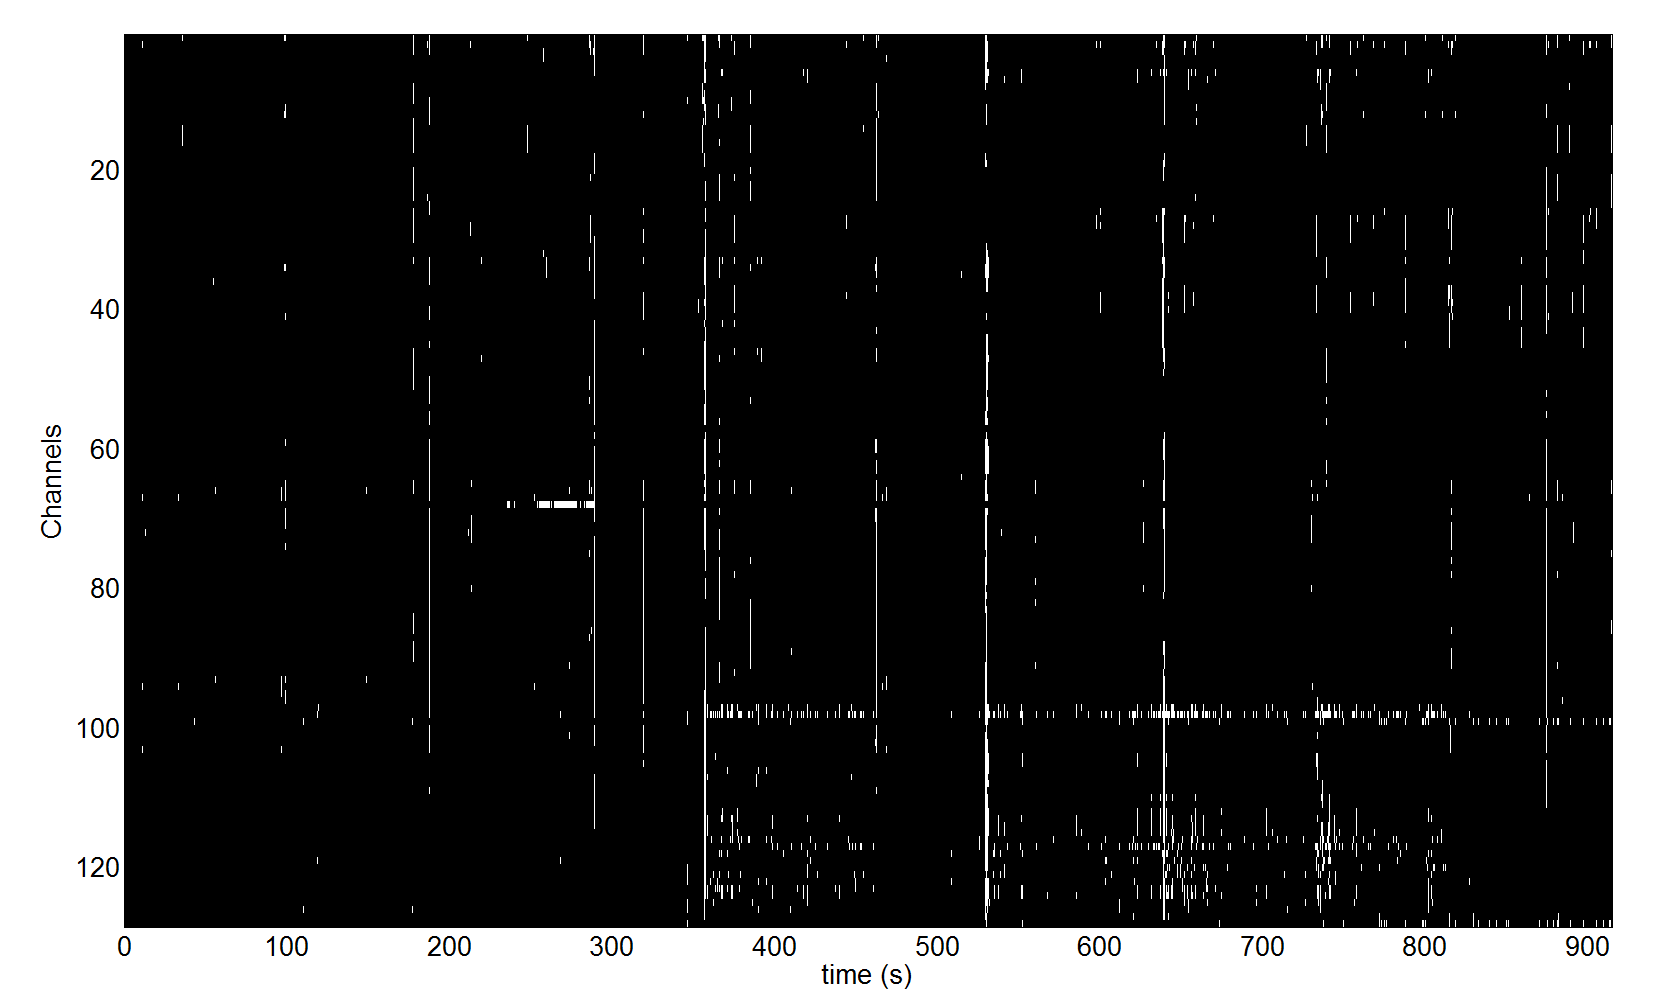
\includegraphics[width=140mm]{meeg_artefact/figure1}
\caption{\em Reviewing marked artefacts \label{artefact_fig1}}
\end{center}
\end{figure}

We can see in the figure that there were several times when some event affected almost all the channels and there is also a group of channels where these events occur more frequently than in other channels especially in the second half of the recording. This is probably due to muscle activity.  Reviewing this kind of plot can be useful to identify problems with your recording and preprocessing pipeline. In the next sections we will see how this information can be used for subsequent automatic processing.

\section{Trial rejection based on marked artefacts}

Proceed with the low-pass filtering and epoching steps as described in the MMN tutorial chapter. We will assume that you now have the epoched dataset \texttt{efadfMspmeeg\_subject1}. Note that artefact marking can be integrated into the batch pipeline with the other steps. We will not describe this in detail but will leave as an exercise to the reader. 

Open the `Detect artefacts' tool again and choose \texttt{efadfMspmeeg\_subject1.mat} file as input. In `How to look for artefacts' make a new `Method'. You can keep the `All' for `Channel selection' as it will not make a difference in this case. Under `Detection algorithm' choose `Reject trials based on events'. By default all artefact events are used for rejection here but you could also load a custom event list that can be created and saved in the `Prepare' GUI. Now you can run the tool. In the command window it will be reported that there are 319 rejected trials and 1 bad channels: \texttt{D2}. In reality it�s probably unnecessary to reject all these trials but we selected a rather low detection threshold for demonstration purposes. If you now proceed to averaging the generated output file (\texttt{aefadfMspmeeg\_subject1}), trials with artefacts will not be included in the average. 

\section{Explicit artefact exclusion in robust averaging}

Rejecting any trial with an artefact in any of the channels sacrifices a lot of good data.  This can be justified when we want to be conservative and rule out any contribution of the artefacts to our result. An alternative approach is to use robust averaging but this time to explicitly exclude the data marked as bad from the average. This can help, for example, with eye blinks consistently locked to some event in the trial. If there are many such eye blinks, they will not be suppressed by conventional robust averaging. But if we detect them first and remove them from the average, the average can be made eyeblink-free provided that there is sufficient number of trials without eye blinks. To demonstrate this approach, open the `Average' tool. Choose the \texttt{efadfMspmeeg\_subject1.mat} file as input because we do not want to reject trials here. In `Averaging type' switch to `Robust'.  Set `Remove bad data' to `yes'. If you run the tool now data marked as bad will be excluded from the average. It might be a good idea to low-pass filter the average again as robust averaging might introduce high frequency noise back in the data. 

There are many possible ways to combine marking of different artefact types with trial rejection and robust averaging and we hope that our demonstration made the principles sufficiently clear to you to be able to explore them independently. 



\section{Topography-based artefact correction}

If an eye blink occurs almost in every trial, then trial rejection will lead to discarding most of the data. Robust averaging could still work in this situation but only if the eye blinks do not consistently overlap in peri-stimulus time and for every sample eye blinks are only present in small minority of trials. But if, for instance, your subject blinks every time after making a decision in a gambling task, neither method would work. In this case a topography-based artefact correction would help. Note that depending on the experimental question, one could be more or less cautious about this. If you are interested in the activity of orbitofrontal cortex, it would probably be better to make every effort to ensure that eye-blinks are minimised at the recording stage and the remaining ones are completely excluded as any software correction will always leave residuals and it will be difficult to convince your reviewers that these residuals do not confound your experimental effects.

Topography-based correction implemented in SPM is based on principles quite similar to Independent Component Analysis (ICA). However, unlike for ICA there is no need to in the time consuming procedure of estimating physiological and artefactual components based on data statistics. But rather these are provided to the algorithm explicitly by the user. This makes the method faster and easier to use. We have not performed a systematic comparison with ICA but it is likely that for the purposes of eye blink removal the two methods yield very similar results. 

Applying the topography based correction consists of several steps which can be implemented in one batch pipeline. We will again use the MMN dataset as the example and start from filtered and downsampled dataset \texttt{fdfMspmeeg\_subject1}. 

For reasons that will become clear below we might need a forward model for some of the steps we will demonstrate. In principle, however, depending on the settings topography-based artefact correction is also possible without a forward model. Let us start with defining a forward model using the `Head model specification' batch tool (SPM->M/EEG->Source reconstruction menu in batch). Select \texttt{fdfMspmeeg\_subject1} file as input, under `Coregistration' switch to `Sensor locations are already in MNI space' and run the tool. Now we are ready to proceed. 

Select `Detect artefacts' from the `Preprocessing' drop-down menu. Change `Mode' from `Reject' to `Mark'. Select the \texttt{fdfMspmeeg\_subject1.mat} file as input (if you don�t have this file, return to the MMN tutorial chapter and perform the steps described there to obtain it). In `How to look for artefacts' make a new `Method'. In `Channel selection' delete `All(1)', add `Custom channel' and enter `VEOG' for the channel name. If in your own data you do not have an EOG channel any scalp EEG channel or MEG channel with clear eyeblinks can be used for the same pupose. Under `Detection algorithm' choose `Eyeblinks'. Keep the default settings and run the tool. 

\begin{figure}
\begin{center}
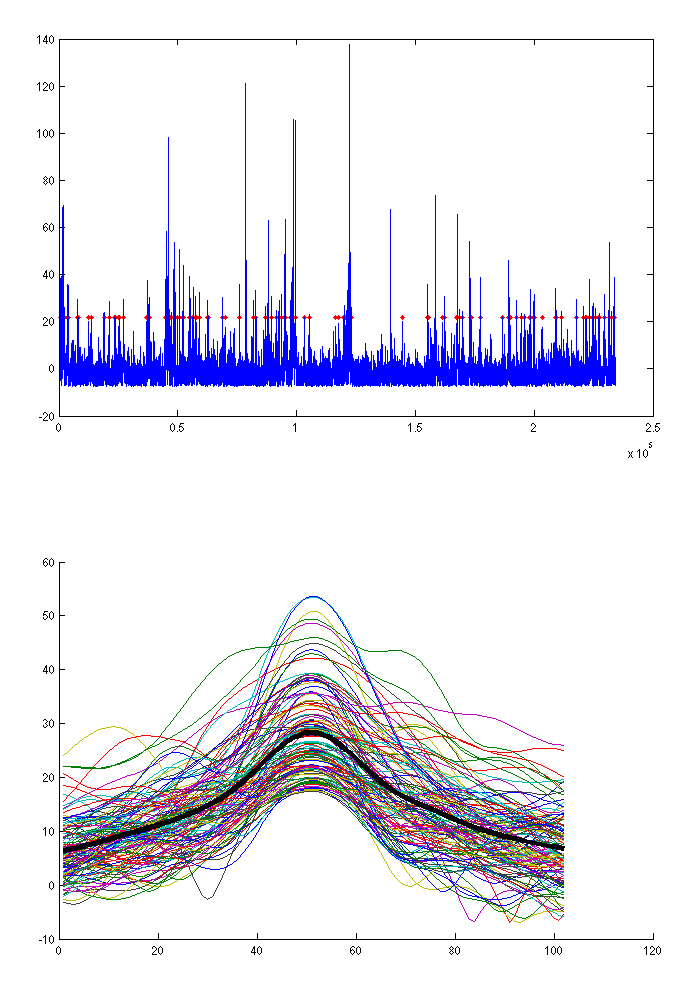
\includegraphics[width=100mm]{meeg_artefact/figure2}
\caption{\em Time points where eye blinks were detected (top) and aligned blink time courses (bottom). \label{artefact_fig2}}
\end{center}
\end{figure}
 
A plot similar to the one from Figure~\ref{artefact_fig2} will appear in SPM graphics window. It shows the points where blinks were detected (top) and aligned blink time courses (bottom). For topography-based correction it is not critical to detect all the blinks, just a representative sample will suffice. If you think too many non-eyeblinks or too few eyeblinks were detected you can adjust the `Threshold' parameter. 

At the next step we will epoch the data around detected eye blinks. Open the `Epoch' tool in `Preprocessing' menu. Choose the \texttt{afdfMspmeeg\_subject1.mat} produced by the previous step as input. In `How to define trials' choose `Define trial'. Set `Time window' to $[-500\ 500]$ and under `Trial definitions' create a new trial with label `Eyeblink', event type `artefact\_eyeblink' and event value `VEOG' (enter this with single quotes). If you remember the artefact events we reviewed in one of the previous sections, the principle is the same here and you would be able to see the eyeblink events in the `Prepare' tool as well (note that `badsamples' will only show them if you look at the VEOG channel as they are specific to that channel). Set `Baseline correction' to `no'. It would also be a good idea to change the default out prefix `e' to `eyeblink' because we might epoch the same file later around stimuli and we would like to avoid a name clash. Now you can run the tool. The output dataset \texttt{eyeblinkafdfMspmeeg\_subject1} will contain epochs with eye blinks. You can review it in the reviewing tool and also average to get an average eye blink. Either epoched or averaged eyeblink file can be used to define eye blink topography. We will use the epoched file as this might enable to also better capture the variability between eyeblinks.

Select `Define spatial confounds' from the `Preprocessing' menu. Use the \texttt{eyeblinkafdfMspmeeg\_subject1} as input. Choose `SVD' under `Mode'. The tool performs singular value decomposition of the trial data to find the spatial patterns that explain most of the variance in the data. What we would like to do now is to keep for artefact template the minimal number of components that are clearly eye-blink related. Since we do not know what that number is we could start with a large number e.g. 4 (set in `Number of components') and run the tool. 

\begin{figure}
\begin{center}
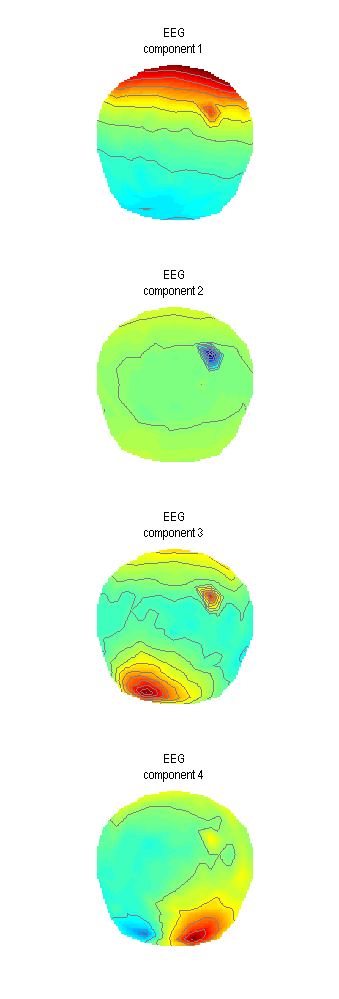
\includegraphics[width=50mm]{meeg_artefact/figure3}
\caption{\em Spatial confounds derived from SVD\label{artefact_fig3}}
\end{center}
\end{figure}
 
Plot such as the one in Figure~\ref{artefact_fig3} will appear in the Graphics window. For averaged-referenced EEG eye-blink related activity appears at the frontal sensors. Thus only the first of the four components is clearly eye-blink related. We could, therefore, only keep that one for our correction. It is possible that with more accurate data preprocessing and removal of other artefacts additional eyeblink components could be extracted. Also for MEG data where head movement change the blink topography over time one component will usually not suffice. For now we will change the `Mode' to `Clear', run the tool again and then return `Mode' to `SVD', set `Number of components' to 1 and run once again. The tool does not produce a separate output file and appends the confound topographies to the same file. Thus clearing is necessary to remove the results of the first run. For your own analysis you might want to explore the typical numbers of eye-blink components for different subjects and runs and decide whether it is safe to always use the same number of check for each file separately. 

The next step is to use the artefact topography we defined using SVD to correct the data we are actually interested in. For this we will need to use `Define spatial confounds' tool once again, but this time our data of interest will be the input, in this case the continuous data file \texttt{afdfMspmeeg\_subject1.mat}. Under `Mode' switch to `SPM M/EEG Dataset' and choose the \texttt{eyeblinkafdfMspmeeg\_subject1} for which we defined confounds above. Run the tool and the confound definition will be copied from \texttt{eyeblinkafdfMspmeeg\_subject1} to \texttt{afdfMspmeeg\_subject1}.

Another way to define spatial confounds is to use the `Eyes' options under `Mode'. The idea there is that three orthogonal dipoles are placed at each eye and their lead-fields are computed using the forward model (that�s one place where you would need one) and used as artefact topographies. If you want to try this option do not forget to clear the previously defined components first. A plot like the one in Figure~\ref{artefact_fig4} will appear.

\begin{figure}
\begin{center}
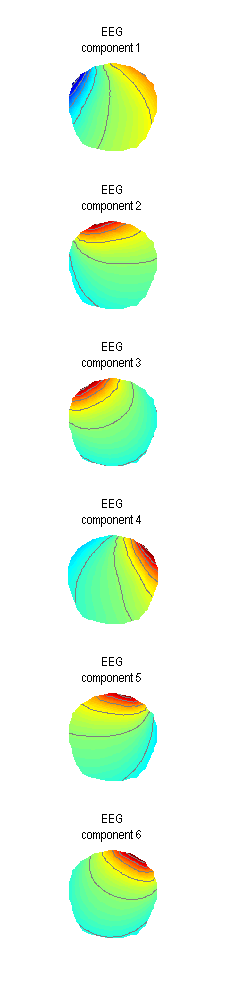
\includegraphics[width=50mm]{meeg_artefact/figure4}
\caption{\em Spatial confounds derived using the EYES option\label{artefact_fig4}}
\end{center}
\end{figure}

You can see here that all the 6 components are expressed at the frontal sensors. This method can also work for removing eye-blinks. Its advantage is that also other activities coming from the eyes can possibly be captured (such as eye movements). However, you will have to sacrifice 6 dimensions of your data which is effectively like removing 6 channels. If you do not have many channels to begin with this can distort your sensor waveforms quite substantially (which might or might not matter depending on the aim of your analysis). Also if the forward model is imprecise it can also happen that some eye-blink related activity will not be removed. Thus where possible the data-driven (SVD) approach is advised.

We are now ready to correct our data. Choose `Correct sensor data' from the `Preprocessing' menu. Choose \texttt{afdfMspmeeg\_subject1.mat} as input. There are two options for correction mode. `SSP' (default) removes everything that can be linearly matched by the artefact topographies from the data, basically making the data orthogonal to the artefact. This method does not require a forward model so if you use SVD in combination with SSP setting you do not have to define a forward model for your data. �Berg� method uses the forward model to define `representative' cortical topographies and keeps the part of the variance that is shared between cortical and artefact topographies, thereby only removing the part that is unlikely to come from the cortex. This method is analogous (though slightly differently implemented) to the one in BESA software (Berg P, Scherg M. Electroencephalogr Clin Neurophysiol. 1994 Mar;90(3):229-41). It requires forward model to be defined.

Artefact correction will produce a new dataset with \texttt{T} prefix: \texttt{TafdfMspmeeg\_subject1.mat}. You might want to run both `SSP' and `Berg' correction changing the default prefix to generate two separate files and compare them later. Review the continuous datasets in the reviewing tool and compare with the uncorrected file to make sure the eyeblinks are indeed gone. You can also epoch and average the corrected files around the eyeblink events and compare the average of the eyeblink dataset we created before (use `Merge' tool to combined different eyeblinks in the same dataset and plot them together). Equivalently, you could apply topography-based correction to the average eyeblink. Since it is a linear operation it does not matter whether you do it on continuous, epoched or averaged data. As a final exercise, you can test the effect of increasing the number of SVD components and compare with the `Eyes' method. 


\section{Fieldtrip visual artefact rejection}

The last tool we are describing here is a compromise between the automatic methods implement in `Detect artefacts' tool and the approach of some very meticulous researchers who examine all their trials by eye. This tool comes from the FieldTrip toolbox (see \footnote{FieldTrip: \url{http://fieldtrip.fcdonders.nl/tutorial/visual_artifact_rejection}}) and SPM only provides an easy interface to it. It can be run by choosing `MEEGTools' from the `Toolbox' menu and then choosing `Fieldtrip visual artefact rejection'. You will first need to choose the input file. For our demonstration here we will use the \texttt{efdfMspmeeg\_subject1} from the MMN tutorial. The tool has three modes that you can choose. We�ll only describe the `Summary' mode here. You can read about the other two at the FieldTrip website (see the link above). You will also be asked to specify the time window you want to look at. This is useful if you have a stimulus artefact and only want to look at part of the peristimulus time. Accept the default which is the whole epoch. A window such as the one in Figure~\ref{artefact_fig5} will appear.

 \begin{figure}
\begin{center}
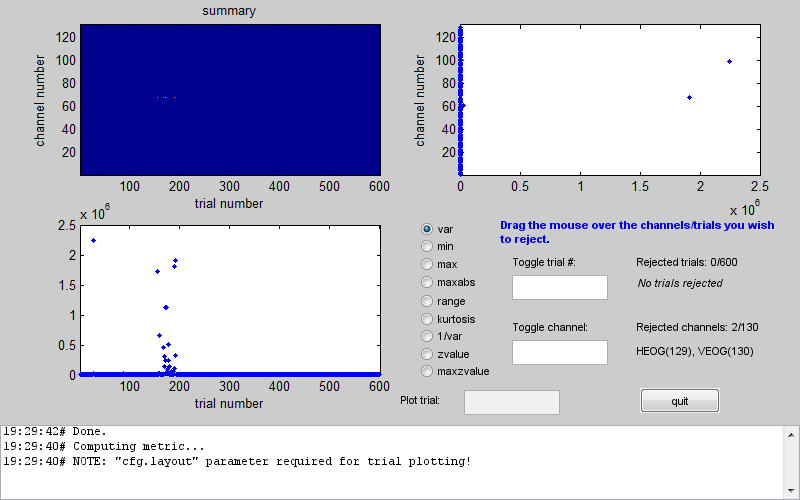
\includegraphics[width=140mm]{meeg_artefact/figure5}
\caption{\em Fieldtrip visual artefact rejection GUI before rejectring trials\label{artefact_fig5}}
\end{center}
\end{figure}

In the centre of the window there is a column of radio buttons that define different measures that can be computed for each channel and trial. When you choose one of these measures the tool computes it for all trials and channels and presents it a channel x trial image at the top left. The plots below and to the right of the image show the maximal values of the measure across channels and across trials respectively. In the above example you can see that between 150th and 200th trial there was a series of trials with unusually high variance. An additional trial with high variance occurred earlier in the recording. If you look at the channel plot you see that there are two channels with higher variance than the others. It is possible that the artefacts are only on those channels and by excluding them you will be able to retain all the trials. Conversely, you could exclude all the bad trials and then the channels will probably not be outliers any more. The choice is in your hands depending on the data and the details of your analysis. Here we�ll exclude trials. This can be done by clicking on the trials plot and dragging the mouse over the points corresponding to the trials we want to exclude while holding the mouse button. After the initial exclusion the plot will be updated and you will see that there are more outliers that are closer to the group than the ones we initially saw but still quite far away. You can exclude them as well in the same manner. By doing this iteratively you can eventually get to a plot like the one in Figure~\ref{artefact_fig6}.

\begin{figure}
\begin{center}
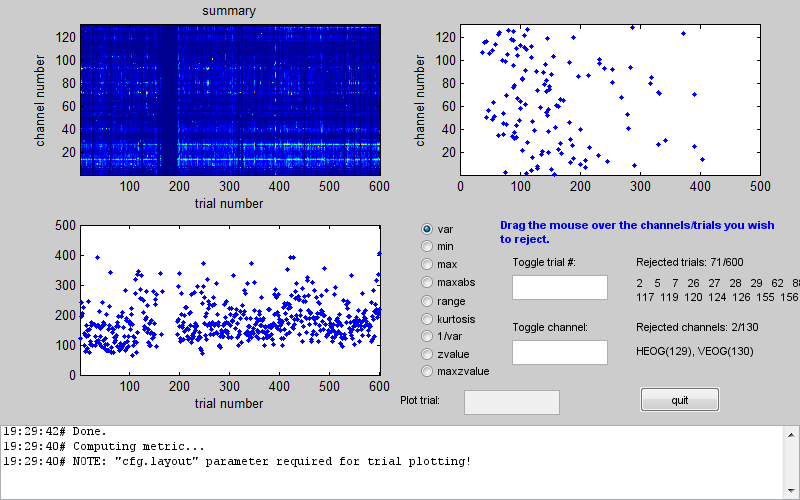
\includegraphics[width=140mm]{meeg_artefact/figure6}
\caption{\em Fieldtrip visual artefact rejection GUI after rejecting outliers\label{artefact_fig6}}
\end{center}
\end{figure}

Here there are no clear outliers in either channels or trials. You could then switch to a different measure which might give you a different picture and keep going until there are no outliers for any of the measures. If you then press the `quit' button your SPM dataset will be updated and the trials and/or channels you chose will be marked as bad. Note that this tool does not create a new dataset so all the changes are done to the dataset you used as input. Make a copy of your dataset first if you want to play with different options. Alternatively you can remove all the bad flags by loading your dataset into the workspace using

\begin{verbatim}
D = spm_eeg_load

and then typing in the commands 

D = badtrials(D, ':', 0);
D = badchannels(D, ':', 0);
save(D);
\end{verbatim}
